\documentclass{beamer}
\mode<presentation>{
  \usetheme{Boadilla}
  \usefonttheme[onlylarge]{structurebold}
  \usefonttheme[stillsansseriflarge]{serif}
  \setbeamerfont*{frametitle}{size=\normalsize,series=\bfseries}
  % \setbeamertemplate{navigation symbols}{}
  \setbeamercovered{transparent}
}
\usepackage[english]{babel}
\usepackage[latin1]{inputenc}
\usepackage{times}
\usepackage[T1]{fontenc}
\usepackage{amsmath}
\usepackage{amssymb}
\usepackage{esint}
\usepackage{hyperref}
\usepackage{tikz}
\usepackage{xkeyval}
\usepackage{xargs}
\usepackage{verbatim}
\usepackage{listings}
\usepackage{multimedia}
\usetikzlibrary{
  arrows,
  calc,
  decorations.pathmorphing,
  decorations.pathreplacing,
  decorations.markings,
  fadings,
  positioning,
  shapes
}

\mode<handout>{
  \usepackage{pgfpages}
  \pgfpagesuselayout{4 on 1}[a4paper,landscape,border shrink=5mm]
  \setbeamercolor{background canvas}{bg=black!10}
}

\newcommand\pgfmathsinandcos[3]{%
  \pgfmathsetmacro#1{sin(#3)}%
  \pgfmathsetmacro#2{cos(#3)}%
}
\newcommand\LongitudePlane[3][current plane]{%
  \pgfmathsinandcos\sinEl\cosEl{#2} % elevation
  \pgfmathsinandcos\sint\cost{#3} % azimuth
  \tikzset{#1/.estyle={cm={\cost,\sint*\sinEl,0,\cosEl,(0,0)}}}
}
\newcommand\LatitudePlane[3][current plane]{%
  \pgfmathsinandcos\sinEl\cosEl{#2} % elevation
  \pgfmathsinandcos\sint\cost{#3} % latitude
  \pgfmathsetmacro\yshift{\cosEl*\sint}
  \tikzset{#1/.estyle={cm={\cost,0,0,\cost*\sinEl,(0,\yshift)}}} %
}
\newcommand\DrawLongitudeCircle[2][1]{
  \LongitudePlane{\angEl}{#2}
  \tikzset{current plane/.prefix style={scale=#1}}
  % angle of "visibility"
  \pgfmathsetmacro\angVis{atan(sin(#2)*cos(\angEl)/sin(\angEl))} %
  \draw[current plane] (\angVis:1) arc (\angVis:\angVis+180:1);
  \draw[current plane,dashed] (\angVis-180:1) arc (\angVis-180:\angVis:1);
}
\newcommand\DrawLatitudeCircleArrow[2][1]{
  \LatitudePlane{\angEl}{#2}
  \tikzset{current plane/.prefix style={scale=#1}}
  \pgfmathsetmacro\sinVis{sin(#2)/cos(#2)*sin(\angEl)/cos(\angEl)}
  % angle of "visibility"
  \pgfmathsetmacro\angVis{asin(min(1,max(\sinVis,-1)))}
  \draw[current plane,decoration={markings, mark=at position 0.6 with {\arrow{<}}},postaction={decorate},line width=.6mm] (\angVis:1) arc (\angVis:-\angVis-180:1);
  \draw[current plane,dashed,line width=.6mm] (180-\angVis:1) arc (180-\angVis:\angVis:1);
}
\newcommand\DrawLatitudeCircle[2][1]{
  \LatitudePlane{\angEl}{#2}
  \tikzset{current plane/.prefix style={scale=#1}}
  \pgfmathsetmacro\sinVis{sin(#2)/cos(#2)*sin(\angEl)/cos(\angEl)}
  % angle of "visibility"
  \pgfmathsetmacro\angVis{asin(min(1,max(\sinVis,-1)))}
  \draw[current plane] (\angVis:1) arc (\angVis:-\angVis-180:1);
  \draw[current plane,dashed] (180-\angVis:1) arc (180-\angVis:\angVis:1);
}
\newcommand\coil[1]{
  {\rh * cos(\t * pi r)}, {\apart * (2 * #1 + \t) + \rv * sin(\t * pi r)}
}
\makeatletter
\define@key{DrawFromCenter}{style}[{->}]{
  \tikzset{DrawFromCenterPlane/.style={#1}}
}
\define@key{DrawFromCenter}{r}[1]{
  \def\@R{#1}
}
\define@key{DrawFromCenter}{center}[(0, 0)]{
  \def\@Center{#1}
}
\define@key{DrawFromCenter}{theta}[0]{
  \def\@Theta{#1}
}
\define@key{DrawFromCenter}{phi}[0]{
  \def\@Phi{#1}
}
\presetkeys{DrawFromCenter}{style, r, center, theta, phi}{}
\newcommand*\DrawFromCenter[1][]{
  \setkeys{DrawFromCenter}{#1}{
    \pgfmathsinandcos\sint\cost{\@Theta}
    \pgfmathsinandcos\sinp\cosp{\@Phi}
    \pgfmathsinandcos\sinA\cosA{\angEl}
    \pgfmathsetmacro\DX{\@R*\cost*\cosp}
    \pgfmathsetmacro\DY{\@R*(\cost*\sinp*\sinA+\sint*\cosA)}
    \draw[DrawFromCenterPlane] \@Center -- ++(\DX, \DY);
  }
}
\newcommand*\DrawFromCenterText[2][]{
  \setkeys{DrawFromCenter}{#1}{
    \pgfmathsinandcos\sint\cost{\@Theta}
    \pgfmathsinandcos\sinp\cosp{\@Phi}
    \pgfmathsinandcos\sinA\cosA{\angEl}
    \pgfmathsetmacro\DX{\@R*\cost*\cosp}
    \pgfmathsetmacro\DY{\@R*(\cost*\sinp*\sinA+\sint*\cosA)}
    \draw[DrawFromCenterPlane] \@Center -- ++(\DX, \DY) node {#2};
  }
}
\makeatother

% not mandatory, but I though it was better to set it blank
\setbeamertemplate{headline}{}
\def\beamer@entrycode{\vspace{-\headheight}}

\tikzstyle{snakearrow} = [decorate, decoration={pre length=0.2cm,
  post length=0.2cm, snake, amplitude=.4mm,
  segment length=2mm},thick, ->]

%% document-wide tikz options and styles

\tikzset{%
  % >=latex, % option for nice arrows
  inner sep=0pt,%
  outer sep=2pt,%
  mark coordinate/.style={inner sep=0pt,outer sep=0pt,minimum size=3pt,
    fill=black,circle}%
}
\tikzset{
  % Define standard arrow tip
  >=stealth',
  % Define style for boxes
  punkt/.style={
    rectangle,
    rounded corners,
    draw=black, very thick,
    text width=8em,
    minimum height=2.5em,
    text centered},
}
\makeatletter
\newbox\@backgroundblock
\newenvironment{backgroundblock}[2]{%
  \global\setbox\@backgroundblock=\vbox\bgroup%
  \unvbox\@backgroundblock%
  \vbox to0pt\bgroup\vskip#2\hbox to0pt\bgroup\hskip#1\relax%
}{\egroup\egroup\egroup}
\addtobeamertemplate{background}{\box\@backgroundblock}{}
\makeatother

% \def\timeleft{15:00->14:55}

\title{NaCs\textsuperscript{\textbf{*}} update}
\date{Sep. 22, 2017}
\author{Yichao Yu}
\institute{Ni Group/Harvard}

\begin{document}

% Give update from NaCs lab
% From Lee's Pizza talk and my title
% Guessed what I'm going to mainly talk about.

% Give slightly more details about what we did and things we learnt.

\begin{frame}{}
  \titlepage
\end{frame}

% Last time, merged without heating Cs
% goal is to make molecules.
% Plan is to use a Raman transition.

\begin{frame}{Making molecules}
  \begin{center}
    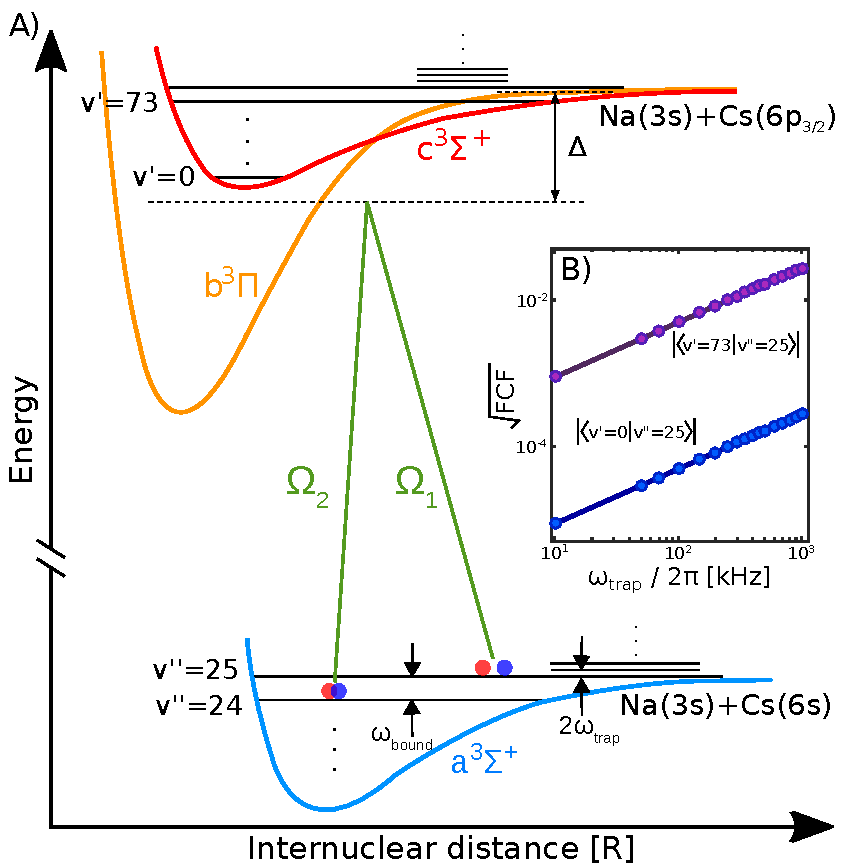
\includegraphics[width=8cm]{../qual/imgs/molecule-formation.pdf}
  \end{center}
\end{frame}

\begin{frame}{Light-assisted collision}
  \begin{columns}
    \column{6.5cm}
    \begin{tikzpicture}
      \draw[->,line width=2] (-0.5, -6.5) -- (5, -6.5) node[right] {$r$};
      \draw[->,line width=2] (-0.5, -6.5) -- (-0.5, 0.8) node[left] {$E$};

      \draw[line width=1,red!70!black]
      plot[smooth,samples=300,domain={1}:{5.5},variable=\x]
      ({\x - 1}, {1 - 3 / \x}) node[right] {S+P};
      \draw[line width=1,blue!70!black] (0, -6) -- (4.5, -6) node[right] {S+S};

      \visible<2>{
        \draw[line width=0.7,->,red] (4, -6) -- (4, 0.9 - 3 / 5);
        \draw[line width=0.7,->,red!50!blue]
        plot[smooth,samples=300,domain={4.9}:{3},variable=\x]
        ({\x - 1}, {0.9 - 3 / \x});
      }

      \visible<3->{
        \draw[line width=1,<-,red] (2, 1.1 - 3 / 3) -- (1, 0.4) node[left] {$\dfrac{1}{r^3}$};
      }
    \end{tikzpicture}
    \column{5cm}
    \begin{center}
      \visible<3->{
        \begin{align*}
          V_{Cs+Na}\propto&\dfrac{1}{r^6}\\
          d_{Cs,S\rightarrow P}\approx&11.4D\\
          V_{Cs+Cs}(100\mathrm{nm})\approx&4MHz\\
          V_{Cs+Na}(5\mathrm{nm})\approx&4MHz
        \end{align*}
      }
      \vspace{-0.6cm}
      \visible<4->{
        \begin{block}{Conclusion}
          Photo association between Na and Cs requires much higher intensity.
        \end{block}
      }
    \end{center}
  \end{columns}
\end{frame}

\begin{frame}{Two body loss}
  \begin{center}
    \only<1>{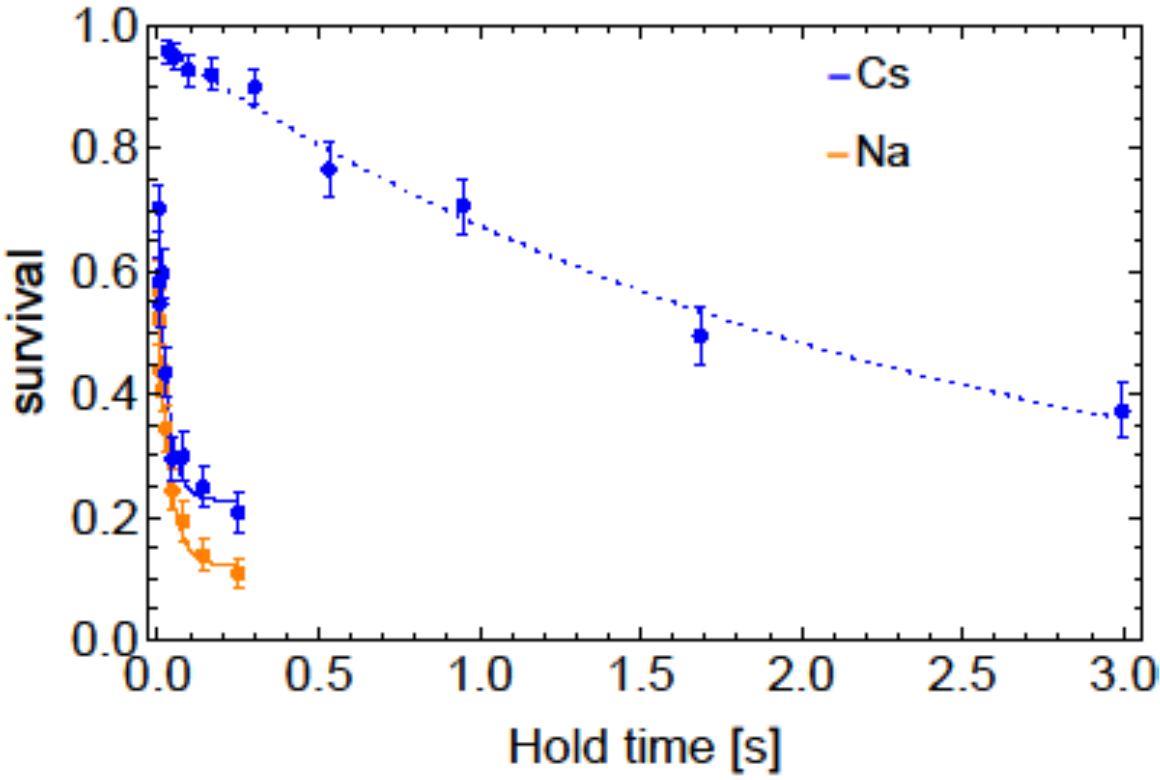
\includegraphics[width=11cm]{imgs/two-body.png}}
    \only<2>{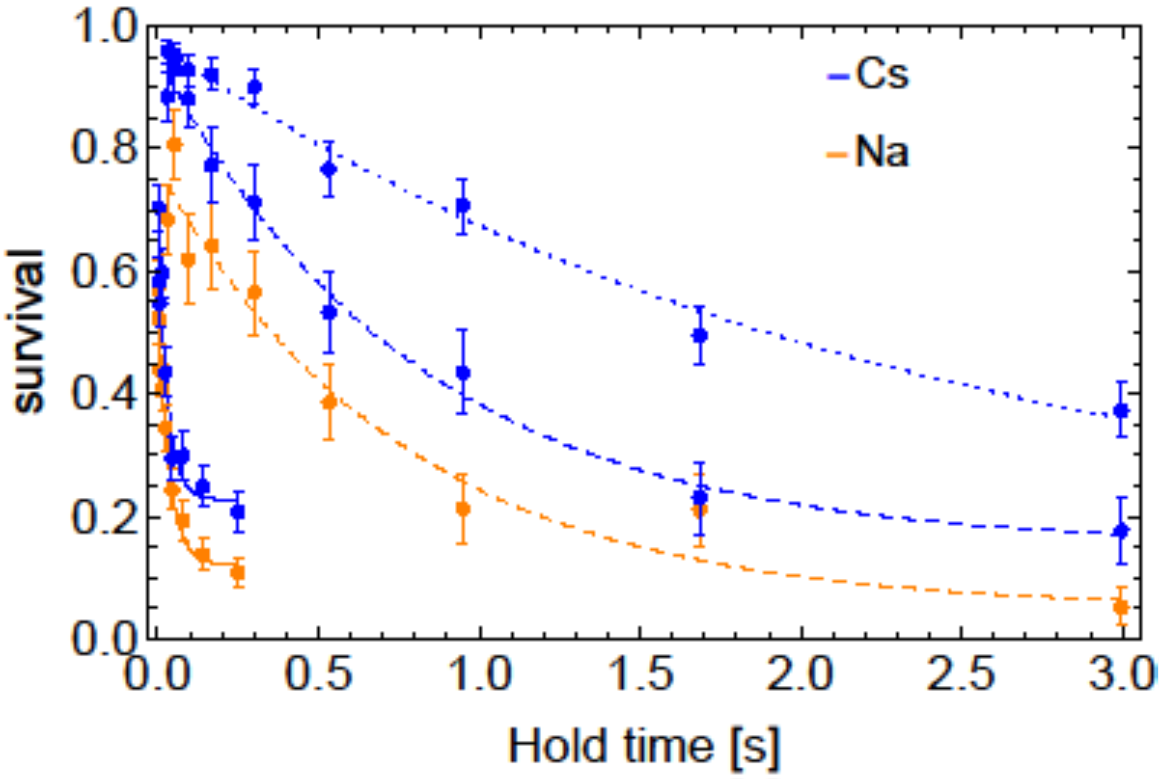
\includegraphics[width=11cm]{imgs/two-body-fixed.png}}
  \end{center}
\end{frame}

\begin{frame}{Photo association}
  \begin{columns}
    \column{6.5cm}
    \visible<2->{
      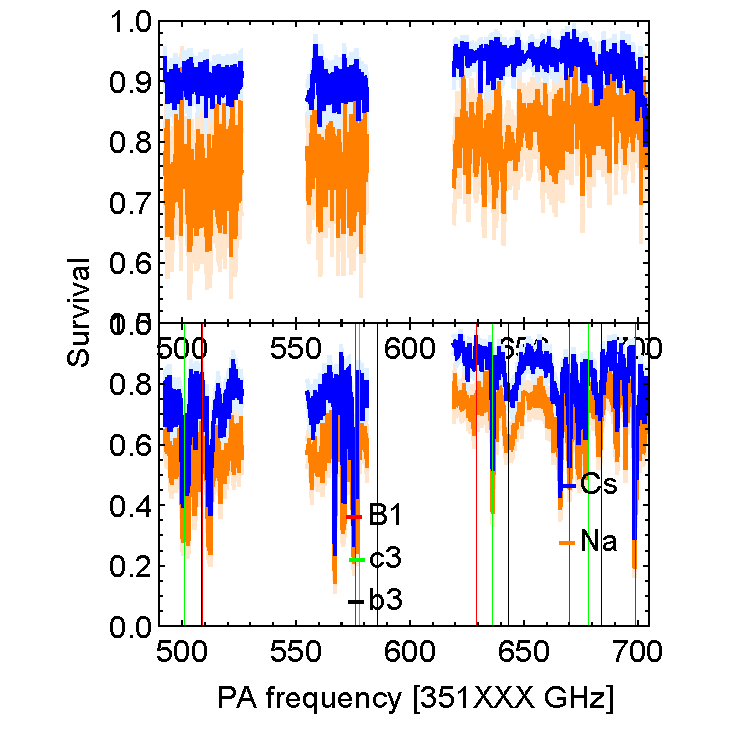
\includegraphics[width=6.5cm]{imgs/PAspectrum.pdf}
    }
    \column{5.5cm}
    \visible<1->{
      \begin{tikzpicture}
        \node[below left] at (0, 0) {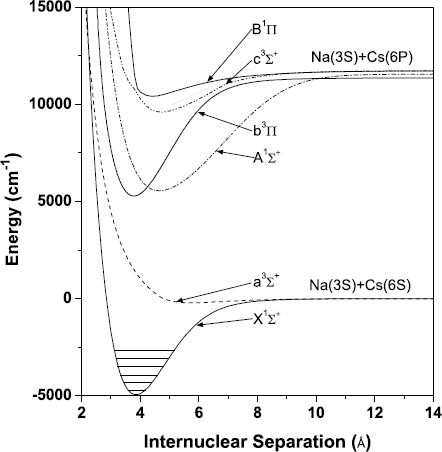
\includegraphics[width=5.5cm]{imgs/PEC.png}};
        \draw[line width=1,<-,blue] (-0.3, -0.8) -- (-0.8, 0.3) node[above] {D1 + D2};
      \end{tikzpicture}
    }
  \end{columns}
\end{frame}

\begin{frame}{Current/next step}
  \begin{columns}
    \column{6cm}
    \begin{itemize}
    \item Get atoms cold again
    \item Prepare hyperfine state
    \item Find molecular ground state
    \end{itemize}
    \includegraphics[5.5cm]{}
    \column{6cm}
  \end{columns}
\end{frame}

\end{document}
